\section{Punto en una Circunferencia}

\subsection{Definición}
El objetivo de este problema de la ingeniería es determinar la inclusión de un punto T, definido por sus coordenadas $(x_2, y_2)$, en el área de una circunferencia específica. Esta posee un centro en el punto C, con coordenadas $(x_1, y_1)$, y un radio de longitud $r$. Se evalúa si el punto T se encuentra dentro del perímetro de la circunferencia o si, por el contrario, se ubica fuera de dicho perímetro

\begin{equation}
\text{distancia} = \sqrt{(x_2 - x_1)^2 + (y_2 - y_1)^2}
\end{equation}

Resulta necesario llevar a cabo una comparación exhaustiva entre la distancia que separa al centro de la circunferencia y el punto T, y la longitud del radio. Si la distancia obtenida resulta ser menor o igual a la longitud del radio, se puede concluir que el punto T se encuentra ubicado dentro de los límites de la circunferencia. Por el contrario, si la distancia es mayor a la longitud del radio, se establece que el punto T se encuentra situado en una posición exterior con respecto a la circunferencia.

\subsection{Descripción del problema}

Dada una circunferencia con centro en el punto C con coordenadas $(x_1, y_1)$ y radio $r$, evaluar si un punto T con coordenadas $(x_2, y_2)$ está dentro del área de la circunferencia.

\subsection{Diseño de solución}

La distancia entre el centro $C$ y el punto $T$ se calcula utilizando la fórmula de la distancia entre dos puntos en el plano la cual se define como anteriormente en la ecuación 5.

 \begin{figure}[h!]
\centering
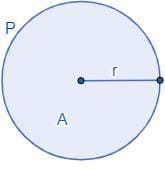
\includegraphics[width=6cm]{imagen/Imagen de WhatsApp 2023-11-23 a las 21.07.09_8c5cc9f6.jpg}
\caption{Gráfica de una circunferencia}
\label{fig:grafica}
\end{figure}

\subsection{Desarrollo de solución}

\lstset{
  language=Java,
  basicstyle=\ttfamily,
  keywordstyle=\bfseries,
  commentstyle=\itshape,
  showstringspaces=false,
  columns=flexible,
  frame=single,
  numbers=left,
  numberstyle=\tiny,
  breaklines=true,
  captionpos=b
}

\begin{javaCode}




        Scanner scanner = new Scanner(System.in);

        System.out.println("Ingrese la coordenada x1");
        double x1 = scanner.nextDouble();
        System.out.println("Ingrese la coordenada y1");
        double y1 = scanner.nextDouble();

        System.out.println("Ingrese el radio de la circunferencia (r):");
        double r = scanner.nextDouble();

        System.out.println("Ingrese la coordenada a evaluar con el punto x2");
        double Tx2 = scanner.nextDouble();
        System.out.println("ingrese la coordenada a evaluar con el punto y2");
        double Ty2 = scanner.nextDouble();

        double distancia = Math.sqrt(Math.pow(Tx2 - x1, 2) + Math.pow(Ty2 - y1, 2));

        if (distancia <= r) {
            System.out.println("El punto se encuentra dentro del area de la circunferencia.");
        } else {
            System.out.println("El punto esta fuera del area de la circunferencia.");
        }
    }
    
}

\end{javaCode}
\\
\subsection{Depuración y pruebas}
En el cuadro 2 se muestran los resultados obtenidos al compilar el código en JAVA de este problema.
\begin{table}[!ht]
\label{T:equipos}
\begin{center}
\begin{tabular}{| c | c | c | c | c | c |}
\hline
\textbf{$x_1$} & \textbf{$y_1$} & \textbf{$r$} & \textbf{$x_2$} & \textbf{$y_2$} & \textbf{Afuera o Adentro}\\
\hline
1 & 2 & 4 & 2 & 1 & Adentro \\
3 & 4 & 2 & 2 & 1 & Afuera \\
1 & 6 & 4 & 4 & 5 & Adentro \\
7 & 4 & 10 & -5 & -3 & Afuera\\
-4 & -5 & 6 & -7 & -8 & Adentro\\
\hline
\end{tabular}
\caption{Tabla de corridas.}
\end{center}
\end{table}
